Mole.io utilizza una configurazione di MongoDB in grado di garantire un alto grado di scalabilit� del sistema e, contemporaneamente, un ottimo livello di affidabilit�. La configurazione utilizzata prevede l'uso di due funzionalit� fornite da MongoDB: lo \textit{sharding} ed i \textit{replica-set}.

\subsubsection{Sharding}

Lo sharding � una funzionalit� che ideata per garantire una \textit{scalatura orizzontale} del database. Essa consiste nella suddivisione dei dati su diversi server, detti \textit{shard}. MongoDB utilizza questa funzionalit� per distribuire grandi \textit{data-set} su un numero variabile di macchine e garantire un alto \textit{throughput} del database.

Ogni shard � un database indipendente, che, in collaborazione con altri shard all'interno della stessa configurazione, concorre a formare un'unica istanza del database: un \textit{cluster}.

L'obiettivo dello \textit{sharding} � la riduzione del carico di lavoro su ogni database. Al crescere del numero di shard presenti all'interno del medesimo cluster, infatti, il numero di operazioni a carico di ogni singolo server, si riduce. Come conseguenza, si ottengono un incremento della capacit� totale del database e un incremento del throughput del sistema.

Al fine di distribuire i dati sui diversi server, � necessaria una politica di scelta dello shard di destinazione. MongoDB offre la possibilit� di definire una \textit{shard key}, cio� una chiave identificativa di un singolo documento, che permette al database di identificare lo shard che dovr� contenere il dato.

MongoDB suddivide i valori delle chiavi di shard in \textit{chunk} e distribuisce i chunk sui diversi server. La suddivisione � operata esclusivamente creando partizioni sull'insieme di valori delle chiavi di shard e assegnando a ciascuna partizione un server ospitante.

La distribuzione dei chunk all'interno dei diversi shard, assicura un bilanciamento del carico di lavoro di ogni server all'interno del cluster. MongoDB utilizza due processi in background per garantire il bilanciamento del cluster:
\begin{description}
\item[splitting] � un processo che evita la crescita eccessiva dei chunk. Si occupa, infatti, di tenere costantemente monitorata la dimensione di ogni chunk, quando uno di essi cresce oltre un limite preconfigurato, lo suddivide in due chunk pi� piccoli. Le eventuali suddivisioni avvengono dopo operazioni di \textit{insert} e \textit{update} e non implicano alcuno spostamento di chunk.
\item[balancer] ha il compito di eseguire la migrazione dei chunk da uno shard ad un altro. Quando la distribuzione dei chunk nei diversi server � sbilanciata, questo processo sposta i chunk contenuti in shard pi� popolati verso shard con \textit{slot} liberi, mantenendo il pi� possibile costante il numero di chunk per shard.
\end{description}

Tra i vantaggi forniti dallo sharding, � possibile annoverare anche un miglioramento delle performance in scrittura. L'aumento della velocit� di scrittura si ottiene come conseguenza della politica di \textit{locking} utilizzata dal database, introdotta nella sezione \ref{Command_query_responsibility_segregation}. I write-lock di MongoDB permettono di eseguire una operazione di scrittura per volta, accodando tutte le altre richieste di inserimento o aggiornamento dei dati. In caso di configurazione cluster, il write-lock avviene a livello di singolo shard. I diversi server possono quindi eseguire una reale parallelizzazione delle operazioni, ottenendo un incremento della velocit� di scrittura globale all'interno del cluster.

\subsubsection{Replica Set}

L'alta affidabilit� di MongoDB � garantita ridondando i dati, mantenendo, quindi, pi� copie dello stesso documento all'interno di server differenti. Nel caso di guasto ad uno dei server e di perdita del dato originale, il sistema � in grado di fornire una copia valida dell'informazione richiesta, ottenendola da un server attivo.

Un Replica Set � un insieme di istanze di MongoDB contenenti gli stessi dati. Uno dei server � definito \textit{primary} e riceve dai client le richieste di scrittura. Il primary esegue l'aggiornamento del suo \textit{data-set} locale e, successivamente, inoltra le richieste verso i \textit{secondary} server, in modo che anch'essi possano mantenere una copia aggiornata dei dati. 

In caso di interruzione del servizio di un server primary, i secondary restanti indicono una votazione per l'elezione automatica di un nuovo primary.

In alcuni casi, la configurazione con Replica Set, pu� essere utilizzata per incrementare la capacit� di lettura dei dati. I client, infatti, possono inviare richieste di lettura dei dati a server differenti, ottenendo cos� una parallelizzazione delle operazioni. Nel caso di cluster distribuiti a livello \textit{world-wide} � possibile, inoltre, configurare il Replica Set in modo da \textit{avvicinare} le copie di dati alla zona di maggiore fruizione, ottenendo, di conseguenza, un incremento delle performance.

\subsubsection{MongoDB in Produzione}

L'utilizzo di MongoDB in produzione, presuppone una combinazione delle funzionalit� di Sharding e Replica Set. In configurazioni di produzione, infatti ogni shard � un Replica Set, questo approccio permette di ottenere un cluster in grado di fornire consistenza dei dati e, al tempo stesso, alta affidabilit�.

Uno sharded cluster MongoDB possiede le seguenti componenti:
\begin{description}
\item[Shard] rappresentano i server di \textit{storage} veri e propri. Ogni shard � un Replica Set gestito da processi chiamati \verb|mongod|. 
\item[Query Router] sono implementati da un \textit{demone} di sistema chiamato \verb|mongos| e si occupano di interfacciare i client con l'intero cluster. A fronte di ogni richiesta di scrittura o lettura, redirigono le operazioni al cluster di competenza, eseguendo, di fatto, il bilanciamento del carico dell'intero sistema. I Query Router sono a loro volta configurati come Replica Set, in modo da garantire alta affidabilit� e non divenire un \textit{single point of failure} dell'intero sistema.
\item[Config Server] possiedono i \textit{metadati} di configurazione dell'intero cluster, cio� i riferimenti ai dati contenuti in ogni shard. I Query Router interrogano i Config Server per identificare il server contenente i dati richiesti dai client. I Config Server sono processi \verb|mongod| equivalenti a quelli utilizzati per gli shard, ma eseguiti con parametri di configurazione specifici, che ne determinano il comportamento.
\end{description}

La figura \ref{fig:shard} mostra schematicamente una possibile configurazione di MongoDB per il deploy in produzione. I server mole e mole-suit contattano i Query Router e interagiscono esclusivamente con i server \verb|mongos|. I Query Router utilizzano quindi le informazioni contenute nei Config Server per identificare uno specifico shard da contattare al fine di completare la richiesta in arrivo dai server di Mole.io

\begin{figure}[h]
\centering
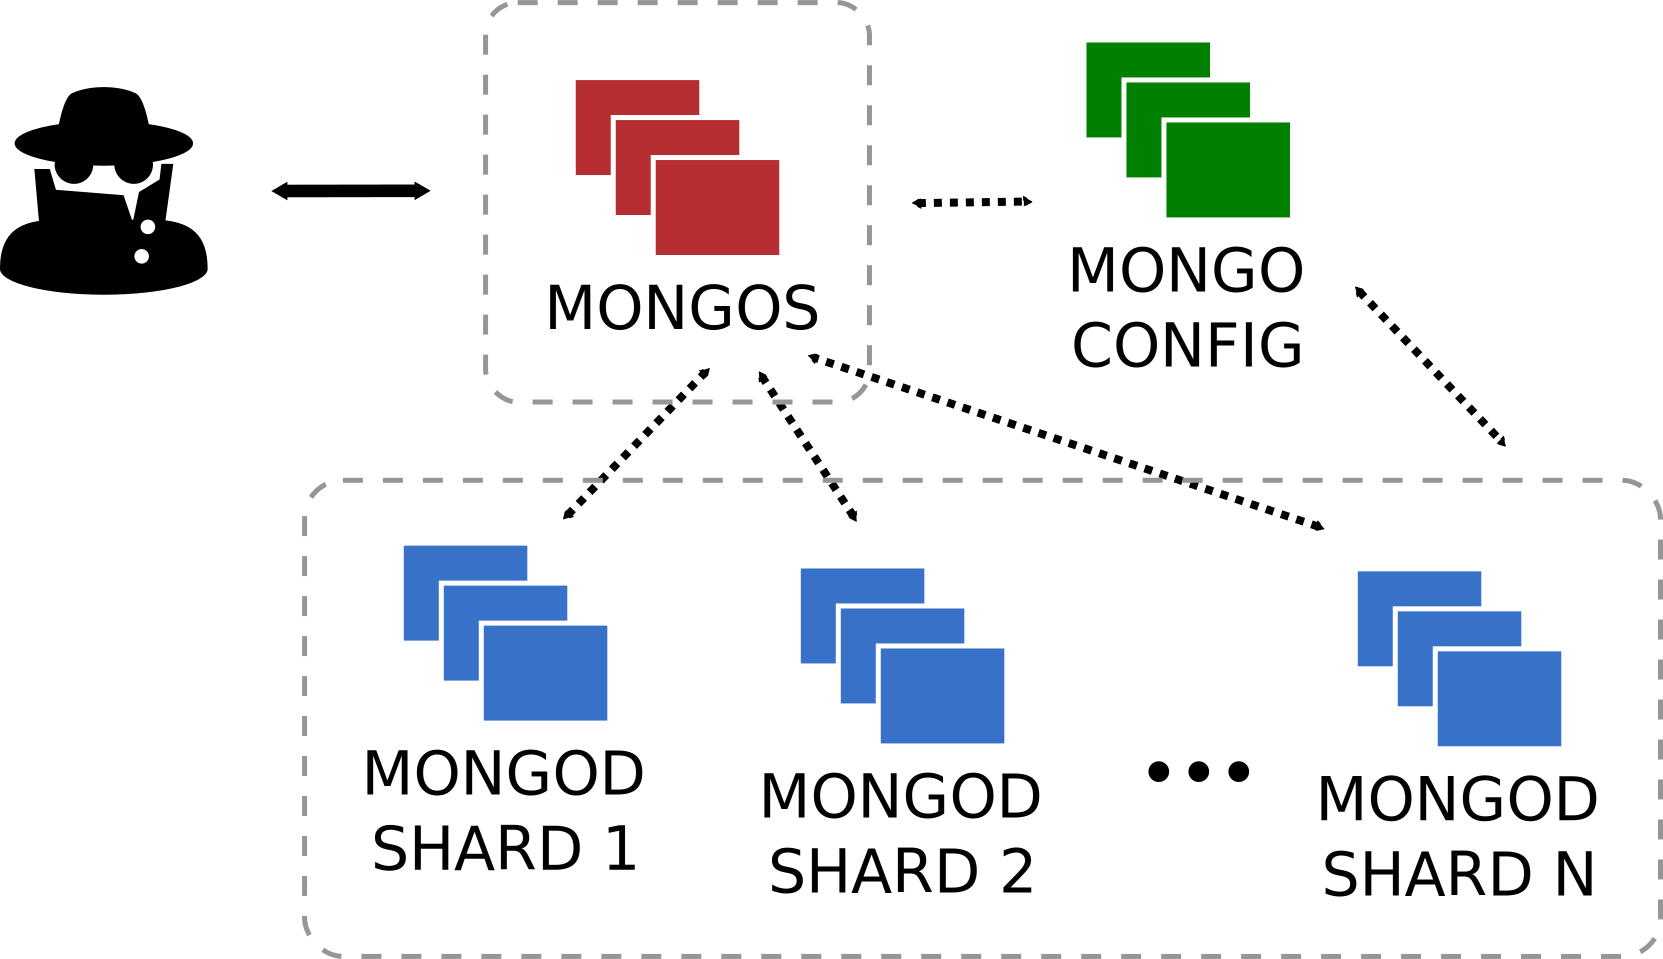
\includegraphics[width=1.0\linewidth]{./img/shard}
\caption[Configurazione di MongoDB per Mole.io]{Configurazione di MongoDB per Mole.io}
\label{fig:shard}
\end{figure}